\documentclass{beamer}
\usepackage[utf8]{inputenc}
\usepackage{graphicx}
\usepackage{amsmath}

\newtheorem{definicion}{Definición}
\newtheorem{ejemplo}{Ejemplo}

%%%%%%%%%%%%%%%%%%%%%%%%%%%%%%%%%%%%%%%%%%%%%%%%%%%%%%%%%%%%%%%%%%%%%%%%%%%%%%%
\title[Búsqueda de raíces]{Búsqueda de raíces}
\subtitle[Método de Newton]{Método de Newton}
\author[Anabel Estévez y Rebeka Luis]{Anabel Estévez Carrillo y Rebeka Luis Hernández}
\date[14-05-14]{La Laguna, 14 de Mayo de 2014}
\usetheme{Madrid}
\definecolor{pantone254}{RGB}{122,59,122}
\definecolor{pantone3015}{RGB}{0,88,147}
\definecolor{pantone432}{RGB}{56,61,66}
\setbeamercolor*{palette primary}{use=structure,fg=white,bg=pantone254}
\setbeamercolor*{palette secondary}{use=structure, fg=white, bg=pantone3015}
\setbeamercolor*{palette tertiary}{use=structure, fg=white, bg=pantone432}


%%%%%%%%%%%%%%%%%%%%%%%%%%%%%%%%%%%%%%%%%%%%%%%%%%%%%%%%%%%%%%%%%%%%%%%%%%%%%%%

\begin{document}

%++++++++++++++++++++++++++++++++++++++++++++++++++++++++++++++++++++++++++++++
\begin{frame}

 %\includegraphics[width=0.15\textwidth]{}
  \hspace*{7.0cm}
  %\includegraphics[width=0.16\textwidth]{}
  \titlepage

  \begin{small}
    \begin{center}
     Técnicas Experimentales \\
     Lenguajes y Sistemas Informácicos \\
     Facultad de Matemáticas \\
     Universidad de La Laguna
    \end{center}
  \end{small}

\end{frame}
%+++++++++++++++++++++++++++++++++++++++++++++++++++++++++++++++++++++++++++++++

%+++++++++++++++++++++++++++++++++++++++++++++++++++++++++++++++++++++++++++++++
\begin{frame}
  \frametitle{Índice}
  \tableofcontents[pausesections]
\end{frame}
%+++++++++++++++++++++++++++++++++++++++++++++++++++++++++++++++++++++++++++++++

\section{Motivación y objetivos}


%++++++++++++++++++++++++++++++++++++++++++++++++++++++++++++++++++++++++++++++
\begin{frame}

\frametitle{Motivación y objetivos}

El objetivo propuesto es obtener los conocimientos necesarios para desarrollar un informe tecnico-científico usando latex, así como:
\begin{itemize}
\item
 La implementación con Python del método de Newton. \pause
\item
 Como se comporta el método de Newton aplicado a la función f(x)=ln x.\pause
\end{itemize}

El procedimiento será descrito en un artículo realizado con el procesador de texto  $LaTeX$ , el cual permite crear documentos con un aspecto profesional y Beamer, una clase de $LaTeX$  para la creación de presentaciones.

\end{frame}
%++++++++++++++++++++++++++++++++++++++++++++++++++++++++++++++++++++++++++++++

\section{Fundamentos teóricos}


%++++++++++++++++++++++++++++++++++++++++++++++++++++++++++++++++++++++++++++++
\begin{frame}

\frametitle{Fundamentos teóricos}
\begin{definicion}
El método de Newton-Raphson es un método iterativo con el que se pueden encontrar aproximaciones de soluciones de ecuaciones no lineales. \pause
\end{definicion}
El método parte de un valor inicial que se introuce en la ecuación:
\begin{center}
$x_n+1 = x_n - \frac{f(x_n)}{f'(x_n)} $ , 
\end{center}
obteniándose así un resultado.Ese resultado se introduce en la misma expresión, obteniendo un nuevo resultado, y así sucesivamente.Si la elección del valor inicial es buena el método proporciona una aproximación a la solución real mejor que la que se haya tenido anteriormente.

\end{frame}
%++++++++++++++++++++++++++++++++++++++++++++++++++++++++++++++++++++++++++++++

\begin{frame}
Para conseguir una buena aproximación se debe tener en cuenta que:
\begin{itemize}
\item
La función debe ser continua y dos veces derivable en un intervalo [a,b].\pause
\item
Se debe escoger un intervalo en el que $f(x)=0$ cumpla el teorema de Bolzano.\pause
\item
$f(a)$ y $f(b)$ tengan signos distintos.
\end{itemize}
\end{frame}
%++++++++++++++++++++++++++++++++++++++++++++++++++++++++++++++++++++++++++++++

\begin{frame}
En conclusión, eligiendo como valor inicial el extremo del intervalo que cumpla: \pause
\begin{center}
$f(a) \times f'(a) > 0$,  o que
$f(b) \times f'(b) > 0$
\end{center}
está asegurado que el método converge a la única solución de la ecuación en [ a,b ].
\end{frame}


\section{Procedimiento experimental}

\subsection{Descripción de los experimentos}
%++++++++++++++++++++++++++++++++++++++++++++++++++++++++++++++++++++++++++++++
\begin{frame}
\frametitle{Descripción de los experimentos}

Se ha redactado un código en el lenguaje de programación $Python$, este cuenta con una función llamada newton que calcula el resultado de aplicar la fórmula de Newton evaluando el error cometido.
Además, el proceso se ejecutará tantas veces como sea necesario para que el error sea menor que un valor prefijado.
\end{frame}
%++++++++++++++++++++++++++++++++++++++++++++++++++++++++++++++++++++++++++++++
\begin{frame}
Ahora bien, el programa se puede ejecutar de dos formas:
\begin{itemize}
\item
Utilizando los parámetros introducidos por el usuario, siempre que estos sean mayores que cero.\pause
\item
Tomando los valores por defecto.
\end{itemize}
\end{frame}
%++++++++++++++++++++++++++++++++++++++++++++++++++++++++++++++++++++++++++++++

\subsection{Descripción del material}

%++++++++++++++++++++++++++++++++++++++++++++++++++++++++++++++++++++++++++++++
\begin{frame}
\frametitle{Descripción del material}
El ordenador empleado cuenta con: 
\begin{itemize}
\item
Un procesador Intel(R) Pentium(R) CPU B960 @ 2.20GHz.\pause
\item
400Gb de disco duro y 6Gb de memoria RAM.\pause
\item
Una velocidad de CPU de 800.000Hz y un caché de CPU de 2048 KB.\pause
\item
El sistema operativo Linux \textit{kubuntu}.\pause

Además, se ha interpretado el código descrito con el intérprete de Python, la versión utilizada ha sido la 2.7.3


\end{itemize}
\end{frame}
%++++++++++++++++++++++++++++++++++++++++++++++++++++++++++++++++++++++++++++++

\subsection{Resultados obtenidos}

%++++++++++++++++++++++++++++++++++++++++++++++++++++++++++++++++++++++++++++++
\begin{frame}
\frametitle{Resultados obtenidos}
Se ha comprobado su precisión dando valores que serán las aproximaciones iniciales de la raíz y se han obtenido los resultados plasmados en la siguiente tabla.

%--------------------------------------------------------------------------
\begin{table}[!ht]
\begin{center}
\begin{tabular}{|c|c|} \hline 
\textbf{Tiempo  } & \textbf{Velocidad} \\ 
\textbf{($\pm$ 0.001 s)} & \textbf{($\pm$ 0.1 m/s)} \\ \hline \hline
1.234 &
67.8
\\
\hline

2.345 &
78.9
\\
\hline

3.456 &
89.1
\\
\hline

4.567 &
91.2
\\
\hline

\end{tabular}
\end{center}
\caption{Resultados experimentales de tiempo (s) y velocidad (m/s)}
\label{tab:1}
\end{table}



\end{frame}
%++++++++++++++++++++++++++++++++++++++++++++++++++++++++++++++++++++++++++++++

\subsection{Análisis de los resultados}
\begin{frame}
Al ejecutar el programa con distintos valores como aproximación inicial de la raíz se observa que en todos los casos se calcula la raíz situada en el punto x=1 con precisión, y por tanto el valor de la función en ese punto es cero.
\begin{figure}[!th]

\begin{center}

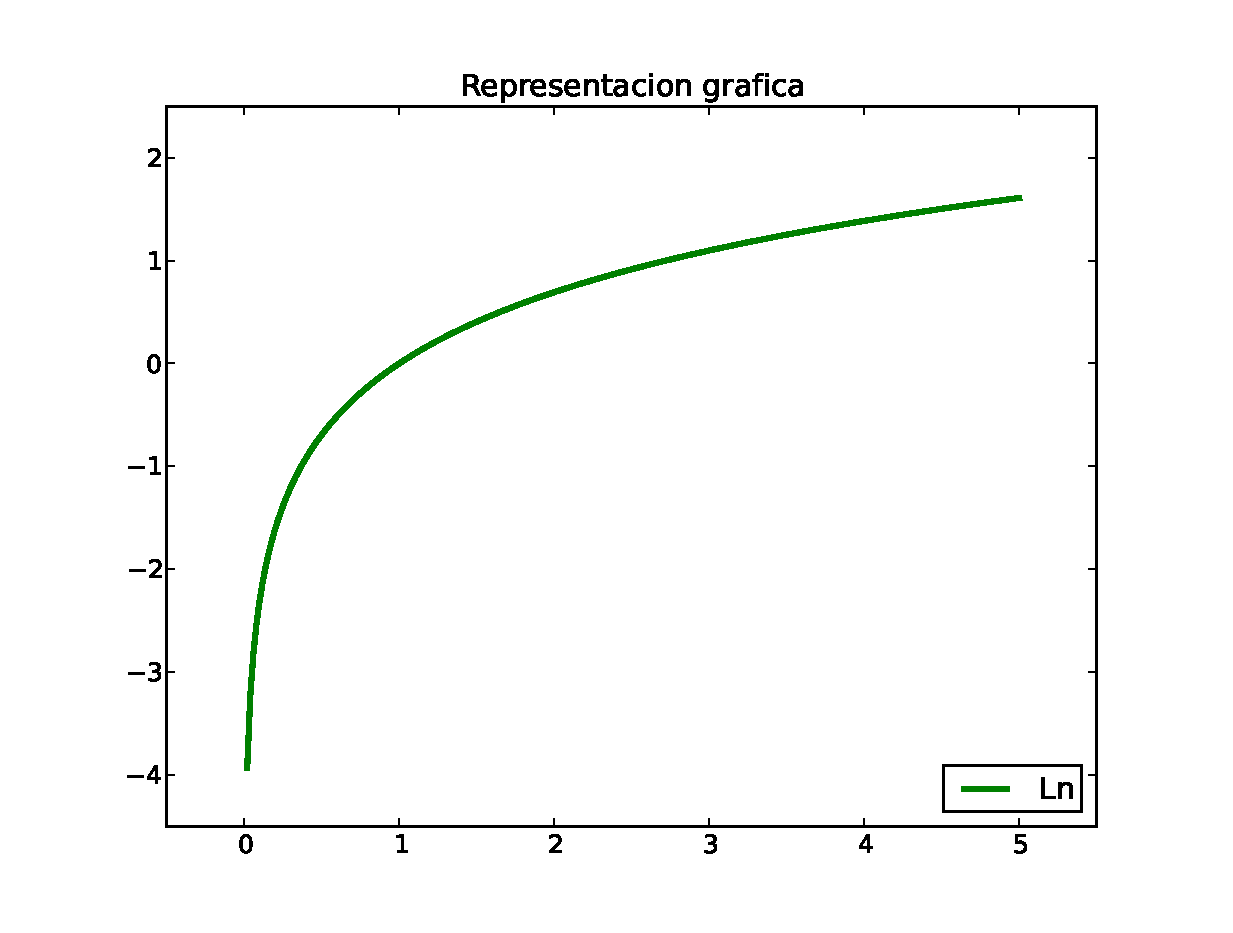
\includegraphics[width=0.75\textwidth]{images/ln-1.eps}

\caption{Ejemplo de figura}

\label{fig:1}

\end{center}

\end{figure}
\end{frame}

\begin{frame}
Cabe destacar que el número de veces que se aplica la fórmula del método de newton, crece cuando la aproximación inicial que introducimos se aleja de la raíz. 
Si se traza una función que represente el número de iteraciones necesarias para calcular las raíces mediante el método de newton para la función $f(x)= log(x)$, se observa que ésta tiene una mayor pendiente cuando nos aproximamos cero
\end{frame}

\begin{frame}
El tiempo de CPU aumenta a medida que se incrementa el valor inicial. Sin embargo, para cualquier valor inicial que se introduzca el tiempo de CPU 
registrado será cero. Así que, para obtener datos al respecto, se ha ejecutado el programa 100000 para cada valor empleando el módulo timeit.


\begin{table}[!h]
\begin{center}
% \label{Mitabla}

\begin{tabular}{cccc}

Valor inicial & Tiempo de CPU al ejecutarse 100000\\

\hline
 
1 & 0.1154410839 \\
2 & 0.5907168388 \\
3 & 0.6773560047 \\
4 & 0.5563027859 \\
5 & 0.7719118595 \\
6 & 0.9161560535 \\
6.5 & 0.8663120270 \\
7 & 0.9962458611 \\
7.35 & 1.3717629910\\ 


\end{tabular}
\end{center}
\caption{Resultados tiempo CPU}
\label{tab:1}
\end{table} 
\end{frame}
\begin{frame}
Estos resultados se han representado en la siguiente gráfica:
\begin{figure}[!th]

\begin{center}

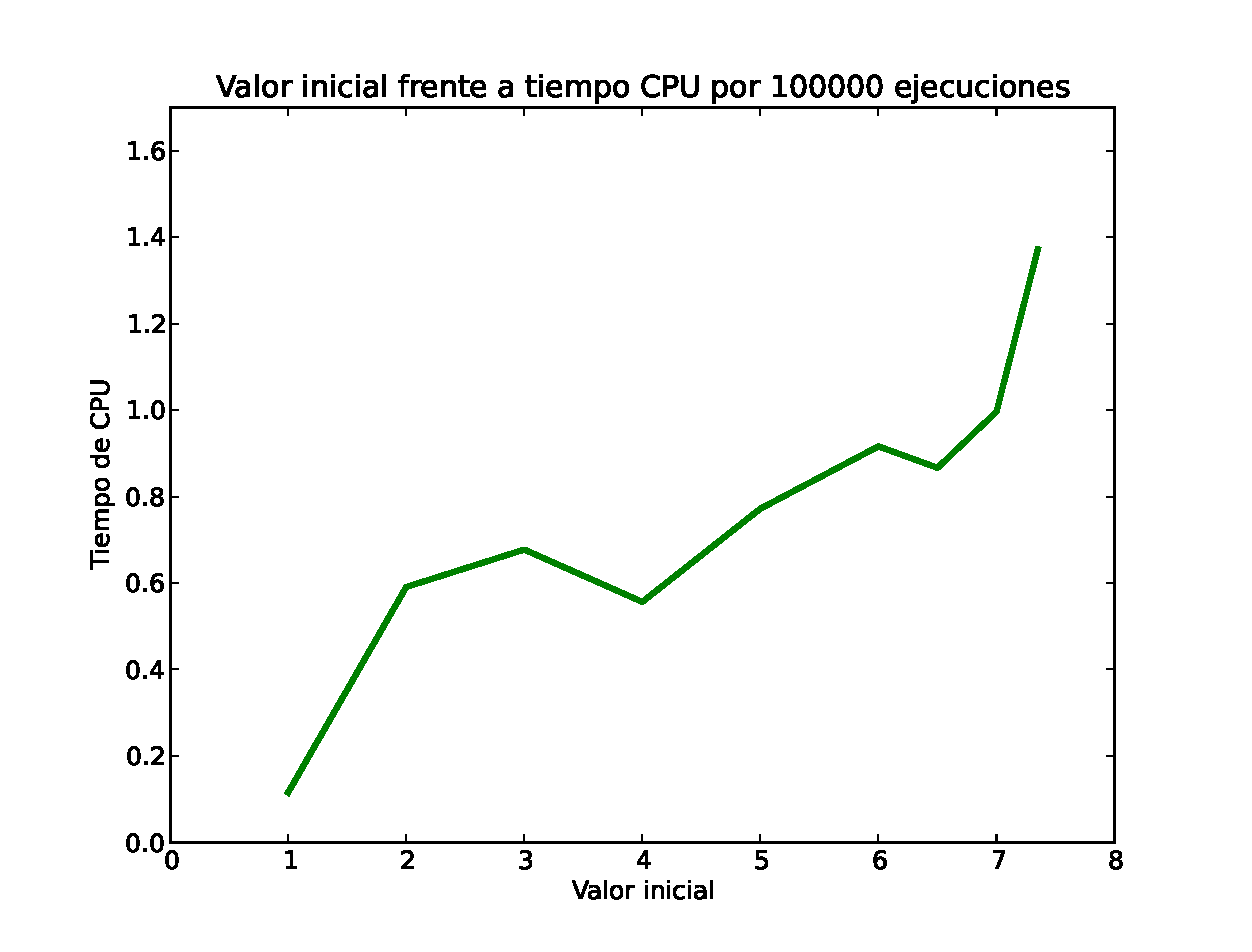
\includegraphics[width=0.75\textwidth]{images/time.eps}

\caption{Tiempo de CPU}

\label{fig:2}

\end{center}

\end{figure} 
\end{frame}

\section{Conclusiones}
\begin{frame}
\frametitle{Conclusiones}
\begin{itemize}
  \item Se ha implementado un código en el lenguaje de programacion Python que consigue resolver de manera precisa la raiz de la función tratada aplicando el método de Newton, si bien el algoritmo diseñado puede ser extrapolado a cualquier otra función.\pause
  \item Si el valor de partida que tomamos como aproximación inicial de la raiz diste de éste, se necesitará aplicar el método de Newton una mayor cantidad de veces para obtener resultados precisos. \pause
  \item El programa diseñado actúa con eficiencia, sin embargo, el tiempo de CPU necesarió será mayor cuando la aproximación inicial de la raíz se aleje de la misma.\pause
\end{itemize}
\end{frame}
\begin{frame}
\begin{itemize}
  \item La elección de un buen valor como aproximación inicial de la raíz es importante para que el programa funcione correctamente. Se han desarrollado los puntos a tener en cuenta para elegir de forma correcta el valor inicial.\pause
  \item A partir del valor 7.389, las aproximaciones en vez de acercarse al 1.00000 se alejan, por lo que llega un momento en el que el valor de x es tan grande, que se produce una división por cero al evaluar la expresión $\frac{log(x)}{(1/x)}$. Por lo tanto, como x es muy grande el cociente $\frac{1}{x}$ tiende a 0 y la división principal provoca el error.
\end{itemize}
\end{frame}

\section{Bibliografía}
%++++++++++++++++++++++++++++++++++++++++++++++++++++++++++++++++++++++++++++++
\begin{frame}
\frametitle{Bibliografía}

\begin{thebibliography}{10}

  \bibitem[Tutotial de python]{python} 
     Tutorial de Python. 
     {\small$http://es.tldp.org/Tutoriales/Python/tut.pdf$}

   
  \bibitem[Tutotial de Latex]{Latex} 
     Tutorial de Latex. 
     {\small $http://www.fing.edu.uy/~canale/latex.pdf$}

  \bibitem[M\'etodo de Newton]{Newton} 
     M\'etodo de Newton. 
     {\small $http://books.google.es/booksid=65JSdxLG4tsec=frontcCICd=0CEUQ6AEwAgv=onepf=false$}
   %  {\small $https://www.youtube.com/watch?v=bghjK1LugSk&index=9&list=FLUEysALfpZLT1lQj4Y5EMtg$}
   
\end{thebibliography}
\end{frame}

%++++++++++++++++++++++++++++++++++++++++++++++++++++++++++++++++++++++++++++++ 

\end{document}














